\documentclass[a4paper,12pt]{article}
\usepackage{ctex}
\usepackage{enumerate}
\usepackage{times}
\usepackage{mathptmx}
\usepackage{amsmath}
\usepackage{amsfonts}
\usepackage{amssymb}
\usepackage{graphicx}
\usepackage{subfigure}
\usepackage{caption}
\usepackage[top=2cm, bottom=2cm, left=2cm, right=2cm]{geometry}
\usepackage{color}
\usepackage{alltt}
\usepackage[T1]{fontenc}

% highlight theme: XCode IDE
\newcommand{\hlstd}[1]{\textcolor[rgb]{0,0,0}{#1}}
\newcommand{\hlnum}[1]{\textcolor[rgb]{0.14,0,1}{#1}}
\newcommand{\hlesc}[1]{\textcolor[rgb]{0,0,0}{#1}}
\newcommand{\hlstr}[1]{\textcolor[rgb]{0.75,0,0}{#1}}
\newcommand{\hlpps}[1]{\textcolor[rgb]{0.45,0.22,0.06}{#1}}
\newcommand{\hlslc}[1]{\textcolor[rgb]{0,0.5,0.11}{#1}}
\newcommand{\hlcom}[1]{\textcolor[rgb]{0,0.5,0.11}{#1}}
\newcommand{\hlppc}[1]{\textcolor[rgb]{0.45,0.22,0.06}{#1}}
\newcommand{\hlopt}[1]{\textcolor[rgb]{0,0,0}{#1}}
\newcommand{\hlipl}[1]{\textcolor[rgb]{0,0,0}{#1}}
\newcommand{\hllin}[1]{\textcolor[rgb]{0.5,0.5,0.5}{#1}}
\newcommand{\hlkwa}[1]{\textcolor[rgb]{0.56,0,0.33}{#1}}
\newcommand{\hlkwb}[1]{\textcolor[rgb]{0.56,0,0.33}{#1}}
\newcommand{\hlkwc}[1]{\textcolor[rgb]{0.56,0,0.33}{#1}}
\newcommand{\hlkwd}[1]{\textcolor[rgb]{0,0,0}{#1}}

\begin{document}
  \title{����~1-11~��ҵ}
  \author{��������ۿԴ \and ѧ�ţ�161240004}
  \date{}
  \maketitle

  \section{[DH] Problem 4.1}
  \begin{enumerate}[(a)]
    \item
    \begin{tabbing}
      ---- \= ---- \= ---- \= ---- \kill
      $S \leftarrow 0$; \\
      for $i$ going from 1 to $N$ do the following: \\
       \> if $A$[$i,1$]$>A$[$A$[$i,2$]$,1$]$$ then $S \leftarrow S+A$[$i,1$]$$;  \\
      output $S$.
    \end{tabbing}
    \item Suppose the root of the binary tree is $R$.
    \begin{tabbing}
      ---- \= ---- \= ---- \= ---- \kill
      $S \leftarrow 0$; \\
      $P \leftarrow R$; \\
      $N \leftarrow$ the content of the first offspring of $R$; \\
      if the content of $R$ $>$ \textbf{get the salary of $N$th employee} then $S \leftarrow S$ + the content of $R$;\\
      while $P$ has a second offspring do the following: \\
       \> $P \leftarrow$ the second offspring of $P$; \\
       \> $N \leftarrow$ the content of the first offspring of $S$; \\
       \> if the content of $P$ $>$ \textbf{get the salary of $N$th employee} then $S \leftarrow S$ + the content of $P$;\\
      output $S$.\\
      \\
      subroutine \textbf{get the salary of $N$th employee} \\
      $T \leftarrow R$; \\
      do the following $N-1$ times: \\
       \> $T \leftarrow$ the second offspring of $T$; \\
      $T \leftarrow$ the second offspring of $T$; \\
      return the content of $T$; \\
    \end{tabbing}
  \end{enumerate}

  \section{[DH] Problem 4.2}
    \begin{enumerate}[(a)]
    \item
    \begin{tabbing}
      ---- \= ---- \= ---- \= ---- \kill
      $S \leftarrow 0$; \\
      call \textbf{add}($T$, 0);\\
      output $S$.\\
      \\
      subroutine \textbf{add}($P$, $x$)\\
       \> $S \leftarrow S + x$; \\
       \> $N \leftarrow 1$; \\
       \> while $P$ has an $N$th offspring do the following: \\
       \> \> call \textbf{add}(the $N$th offspring of $P$, $x+1$); \\
       \> \> $N \leftarrow N+1$; \\
       \> return.
    \end{tabbing}
    \item
    \begin{tabbing}
      ---- \= ---- \= ---- \= ---- \kill
      $S \leftarrow 0$; \\
      call \textbf{count}($T$, 0);\\
      output $S$;\\
      \\
      subroutine \textbf{count}($P$, $x$)\\
       \> if $x = K$ then do the following: \\
       \> \> $S \leftarrow S + 1$; \\
       \> \> return; \\
       \> $N \leftarrow 1$; \\
       \> while $P$ has an $N$th offspring do the following: \\
       \> \> call \textbf{count}(the $N$th offspring of $P$, $x+1$); \\
       \> \> $N \leftarrow N+1$;\\
       \> return.
    \end{tabbing}
    \item
    \begin{tabbing}
      ---- \= ---- \= ---- \= ---- \kill
      $R \leftarrow$ false; \\
      call \textbf{check}($T$, 0); \\
      output $R$. \\
      \\
      subroutine \textbf{check}($P$, $x$)\\
       \> if $x$ is even then do the following: \\
       \> \> if $P$ doesn't have a first offspring then do the following: \\
       \> \> \> $R \leftarrow$ true; \\
       \> \> \> return; \\
       \> $N \leftarrow 1$; \\
       \> while $P$ has an $N$th offspring do the following: \\
       \> \> call \textbf{check}(the $N$th offspring of $P$, $x+1$); \\
       \> \> $N \leftarrow N+1$;\\
       \> return.
    \end{tabbing}
  \end{enumerate}


  \section{[DH] Problem 4.8}
  Suppose that the maximal distance between any two points on a polygon occurs between $M$ and $N$. First, regard $N$ as an arbitrary fixed point, and consider point $M$. \par
  Case 1: $M$ is in the polygon. Extend $NM$ cutting the polygon at $E$ (Figure 2(a)). $NP$ is longer than than $NM$.  \par
  Case 2: $M$ is on one edge of the polygon, but $M$ is not a vertex  (Figure 2(b)). Let the edge where $M$ is on be $AB$. At least one of $\angle NMA$ and $\angle NMB$ is not less than 90 degrees. Assume, WLOG, that $\angle NMA \geq 90 ^\circ$. By the law of sines, we get $NA > NM$. \par
  Now, we have proved that for arbitrary $N$, the length of $NM$ is maximal when $M$ is a vertex of the polygon. Consider point $N$, we can prove that the length of $MN$ is maximal when $N$ is a vertex  of the polygon likewise (Figure 2(c)). Hence, the maximal distance between any two points on a polygon occurs between two of the vertices. \hfill $\square$

  \begin{figure}[htbp]
    \centering
    \subfigure[]{
      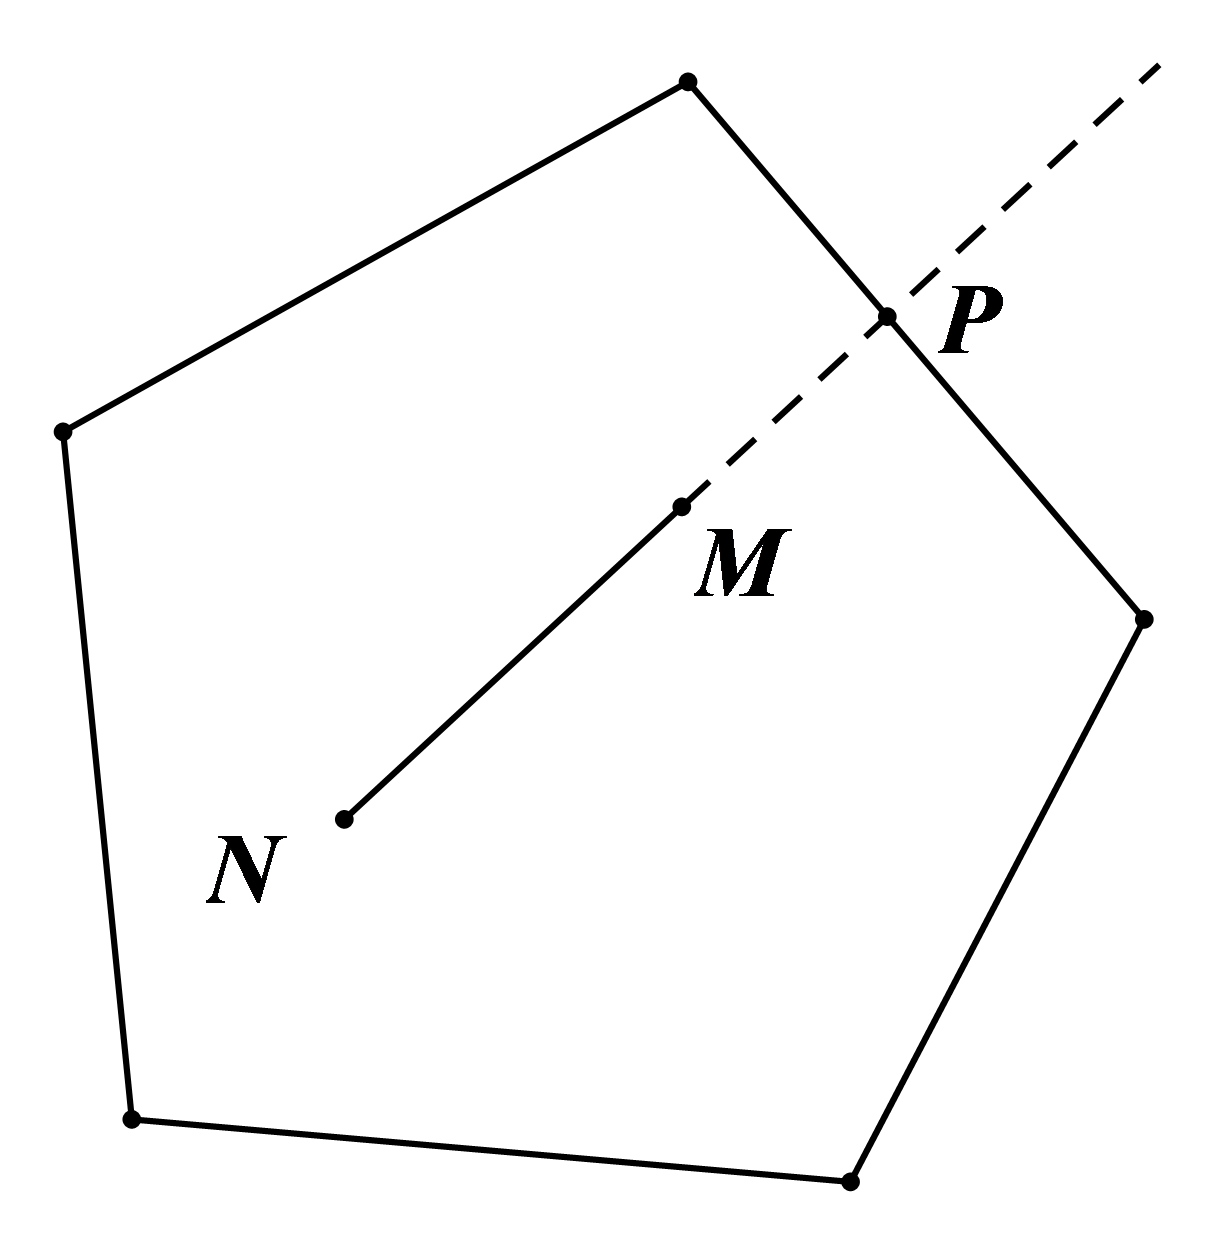
\includegraphics[width=5cm]{figures/fig2_a.png}}
    \subfigure[]{
      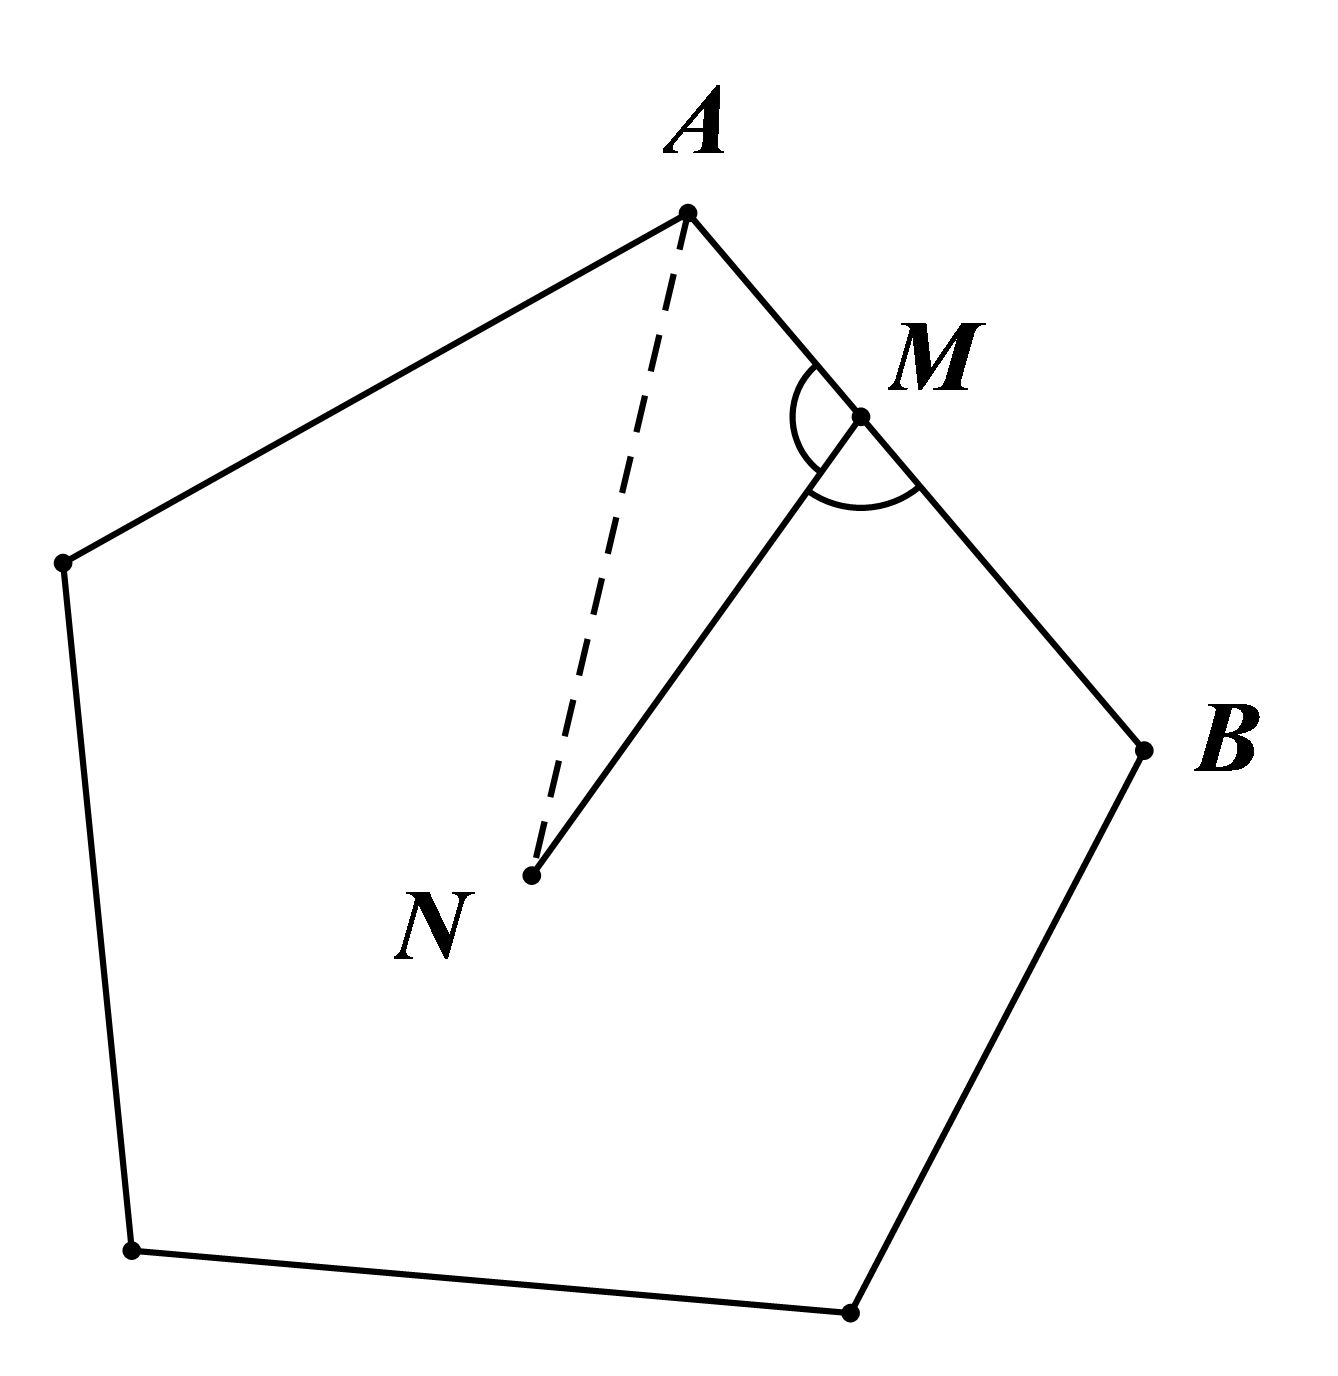
\includegraphics[width=5cm]{figures/fig2_b.png}}
    \subfigure[]{
      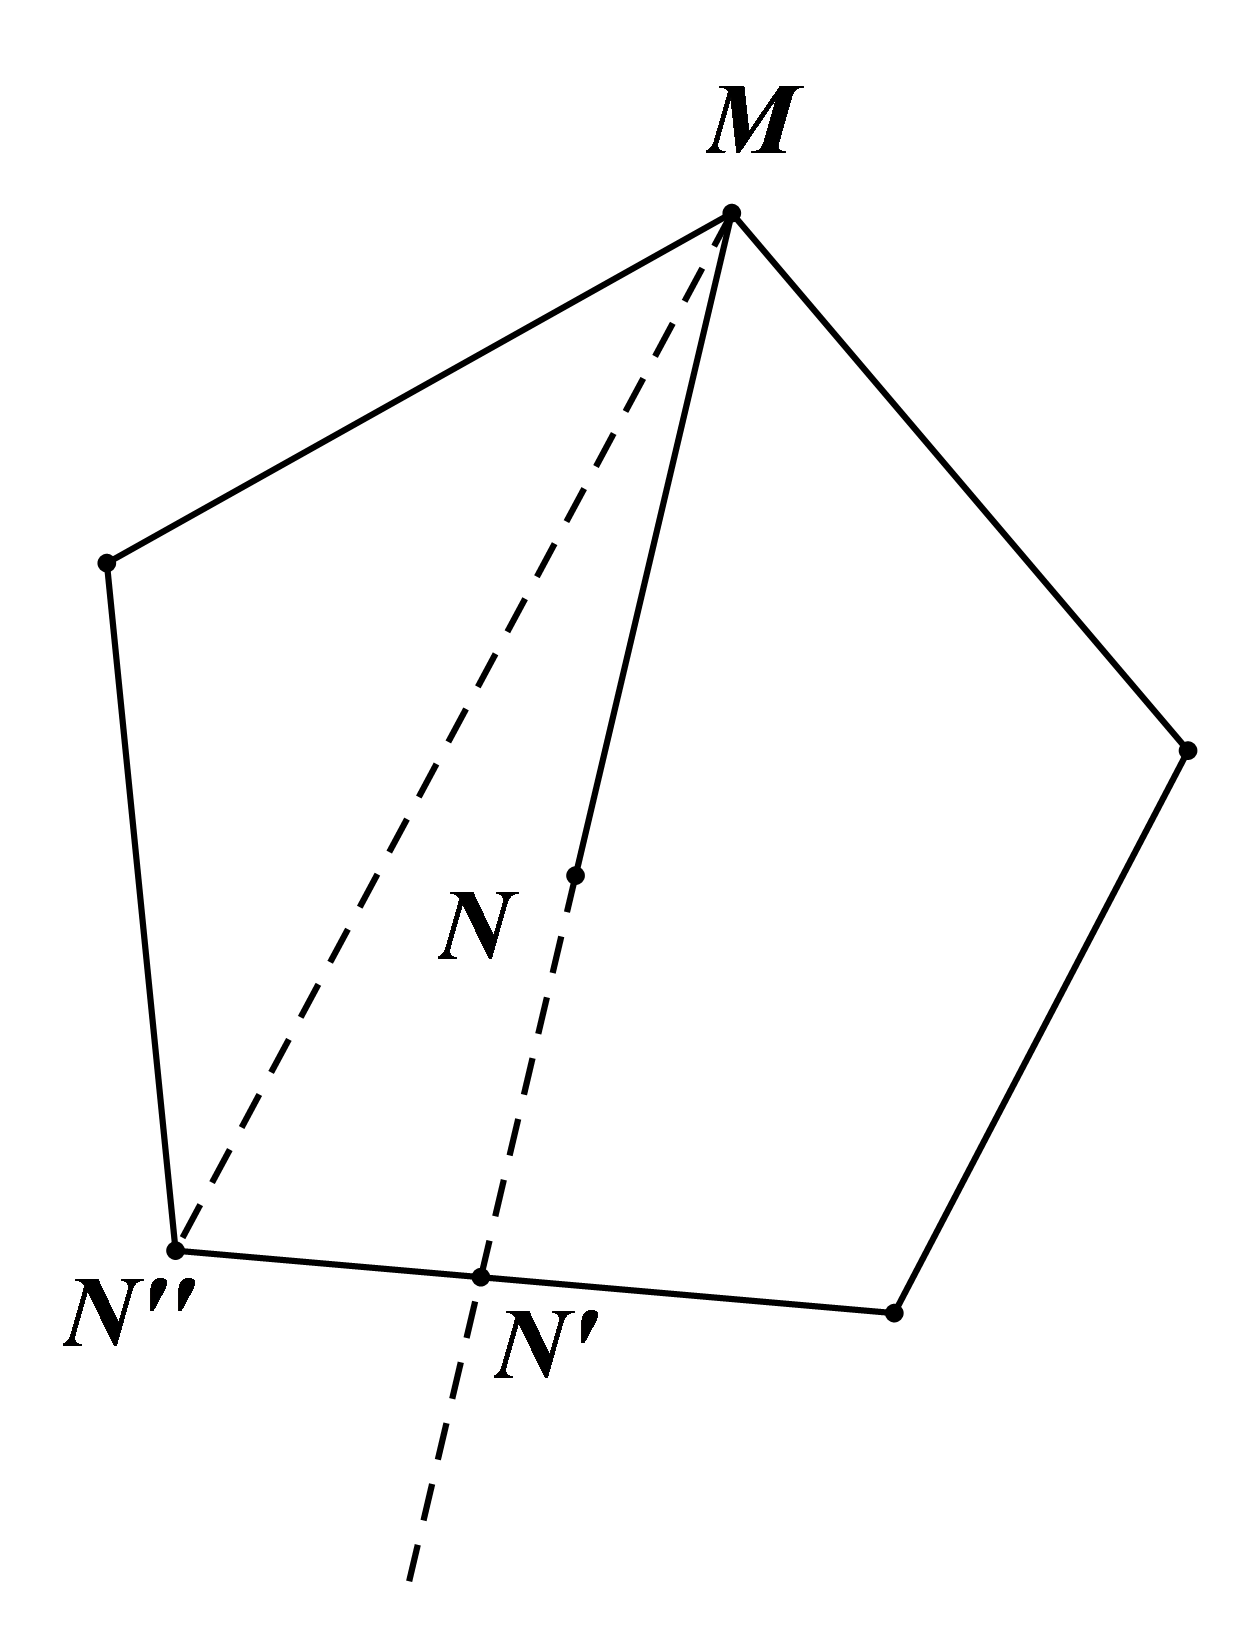
\includegraphics[width=5cm]{figures/fig2_c.png}}
    \caption*{Figure 2: the distance of two points on a polygon}
  \end{figure}

  \section{[DH] Problem 4.9}
 Language: C++ \par
 The first line of the input contains a positive integer $n$, giving the number of the vertices of the polygon. The following $n+1$ lines of the input contains the coordinates of the vertices (in clockwise or counterclockwise order). The x-coordinate and y-coordinate are separated by a space. \par
 The output of the program is a number, the maximal distance of two points on the polygon.
  \par
\newsavebox{\hlboxopenbrace}
\newsavebox{\hlboxclosebrace}
\newsavebox{\hlboxlessthan}
\newsavebox{\hlboxgreaterthan}
\newsavebox{\hlboxdollar}
\newsavebox{\hlboxunderscore}
\newsavebox{\hlboxand}
\newsavebox{\hlboxhash}
\newsavebox{\hlboxat}
\newsavebox{\hlboxbackslash}
\newsavebox{\hlboxpercent}
\newsavebox{\hlboxhat}
\setbox\hlboxopenbrace=\hbox{\verb.{.}
\setbox\hlboxclosebrace=\hbox{\verb.}.}
\setbox\hlboxlessthan=\hbox{\verb.<.}
\setbox\hlboxgreaterthan=\hbox{\verb.>.}
\setbox\hlboxdollar=\hbox{\verb.$.}
\setbox\hlboxunderscore=\hbox{\verb._.}
\setbox\hlboxand=\hbox{\verb.&.}
\setbox\hlboxhash=\hbox{\verb.#.}
\setbox\hlboxat=\hbox{\verb.@.}
\setbox\hlboxbackslash=\hbox{\verb.\.}
\setbox\hlboxpercent=\hbox{\verb.\%.}
\setbox\hlboxhat=\hbox{\verb.^.}
\def\urltilda{\kern -.15em\lower .7ex\hbox{\~{}}\kern .04em}
\noindent
\ttfamily
\hlstd{}\hlppc{\#include\ \usebox{\hlboxlessthan}iostream\usebox{\hlboxgreaterthan}}\hspace*{\fill}\\
\hlstd{}\hlppc{\#include\ \usebox{\hlboxlessthan}cmath\usebox{\hlboxgreaterthan}}\hspace*{\fill}\\
\hlstd{}\hlppc{\#include\ \usebox{\hlboxlessthan}algorithm\usebox{\hlboxgreaterthan}}\hspace*{\fill}\\
\hlstd{}\hlkwa{using\ namespace\ }\hlstd{std}\hlopt{;}\hspace*{\fill}\\
\hlstd{}\hspace*{\fill}\\
\hlstd{}\hlkwb{int\ }\hlstd{n}\hlopt{;}\hspace*{\fill}\\
\hlstd{}\hlkwb{double\ }\hlstd{x}\hlopt{{[}}\hlstd{}\hlnum{1000}\hlstd{}\hlopt{{]},\ }\hlstd{y}\hlopt{{[}}\hlstd{}\hlnum{1000}\hlstd{}\hlopt{{]};}\hspace*{\fill}\\
\hlstd{}\hspace*{\fill}\\
\hlstd{}\hlkwb{double\ }\hlstd{}\hlkwd{dist}\hlstd{}\hlopt{(}\hlstd{}\hlkwb{int\ }\hlstd{i1}\hlopt{,\ }\hlstd{}\hlkwb{int\ }\hlstd{i2}\hlopt{)}\hspace*{\fill}\\
\hlstd{}\hlopt{\usebox{\hlboxopenbrace}}\hspace*{\fill}\\
\hlstd{}\hlstd{\ \ \ \ }\hlstd{}\hlkwa{return\ }\hlstd{}\hlkwd{hypot}\hlstd{}\hlopt{(}\hlstd{x}\hlopt{{[}}\hlstd{i1\ }\hlopt{\%\ }\hlstd{n}\hlopt{{]}\ {-}\ }\hlstd{x}\hlopt{{[}}\hlstd{i2\ }\hlopt{\%\ }\hlstd{n}\hlopt{{]},\ }\hlstd{y}\hlopt{{[}}\hlstd{i1\ }\hlopt{\%\ }\hlstd{n}\hlopt{{]}\ {-}\ }\hlstd{y}\hlopt{{[}}\hlstd{i2\ }\hlopt{\%\ }\hlstd{n}\hlopt{{]});}\hspace*{\fill}\\
\hlstd{}\hlopt{\usebox{\hlboxclosebrace}}\hspace*{\fill}\\
\hlstd{}\hspace*{\fill}\\
\hlstd{}\hlkwb{int\ }\hlstd{}\hlkwd{main}\hlstd{}\hlopt{()}\hspace*{\fill}\\
\hlstd{}\hlopt{\usebox{\hlboxopenbrace}}\hspace*{\fill}\\
\hlstd{}\hlstd{\ \ \ \ }\hlstd{}\hlkwb{double\ }\hlstd{ans\ }\hlopt{=\ }\hlstd{}\hlnum{0}\hlstd{}\hlopt{;}\hspace*{\fill}\\
\hlstd{}\hlstd{\ \ \ \ }\hlstd{}\hlkwb{int\ }\hlstd{j}\hlopt{,\ }\hlstd{k}\hlopt{;}\hspace*{\fill}\\
\hlstd{}\hlstd{\ \ \ \ }\hlstd{cin\ }\hlopt{\usebox{\hlboxgreaterthan}\usebox{\hlboxgreaterthan}\ }\hlstd{n}\hlopt{;}\hspace*{\fill}\\
\hlstd{}\hlstd{\ \ \ \ }\hlstd{}\hlkwa{for\ }\hlstd{}\hlopt{(}\hlstd{}\hlkwb{int\ }\hlstd{i\ }\hlopt{=\ }\hlstd{}\hlnum{0}\hlstd{}\hlopt{;\ }\hlstd{i\ }\hlopt{\usebox{\hlboxlessthan}\ }\hlstd{n}\hlopt{;\ }\hlstd{i}\hlopt{++)}\hspace*{\fill}\\
\hlstd{}\hlstd{\ \ \ \ \ \ \ \ }\hlstd{cin\ }\hlopt{\usebox{\hlboxgreaterthan}\usebox{\hlboxgreaterthan}\ }\hlstd{x}\hlopt{{[}}\hlstd{i}\hlopt{{]}\ \usebox{\hlboxgreaterthan}\usebox{\hlboxgreaterthan}\ }\hlstd{y}\hlopt{{[}}\hlstd{i}\hlopt{{]};}\hspace*{\fill}\\
\hlstd{}\hlstd{\ \ \ \ }\hlstd{j\ }\hlopt{=\ }\hlstd{n}\hlopt{;}\hspace*{\fill}\\
\hlstd{}\hlstd{\ \ \ \ }\hlstd{k\ }\hlopt{=\ }\hlstd{n\ }\hlopt{+\ }\hlstd{}\hlnum{1}\hlstd{}\hlopt{;}\hspace*{\fill}\\
\hlstd{}\hlstd{\ \ \ \ }\hlstd{}\hlkwa{while\ }\hlstd{}\hlopt{(}\hlstd{k\ }\hlopt{\usebox{\hlboxlessthan}\ }\hlstd{}\hlnum{2}\hlstd{}\hlopt{{*}}\hlstd{n}\hlopt{)}\hspace*{\fill}\\
\hlstd{}\hlstd{\ \ \ \ }\hlstd{}\hlopt{\usebox{\hlboxopenbrace}}\hspace*{\fill}\\
\hlstd{}\hlstd{\ \ \ \ \ \ \ \ }\hlstd{}\hlkwa{while\ }\hlstd{}\hlopt{(!(}\hlstd{}\hlkwd{dist}\hlstd{}\hlopt{(}\hlstd{j}\hlopt{,\ }\hlstd{k}\hlopt{)\ \usebox{\hlboxgreaterthan}\ }\hlstd{}\hlkwd{dist}\hlstd{}\hlopt{(}\hlstd{j}\hlopt{,\ }\hlstd{k\ }\hlopt{{-}\ }\hlstd{}\hlnum{1}\hlstd{}\hlopt{)\ \&\&\ }\hlstd{}\hlkwd{dist}\hlstd{}\hlopt{(}\hlstd{j}\hlopt{,\ }\hlstd{k}\hlopt{)\ \usebox{\hlboxgreaterthan}\ }\hlstd{}\hlkwd{dist}\hlstd{}\hlopt{(}\hlstd{j}\hlopt{,\ }\hlstd{k\ }\hlopt{+\ }\hlstd{}\hlnum{1}\hlstd{}\hlopt{)))}\hspace*{\fill}\\
\hlstd{}\hlstd{\ \ \ \ \ \ \ \ \ \ \ \ }\hlstd{k}\hlopt{++;}\hspace*{\fill}\\
\hlstd{}\hlstd{\ \ \ \ \ \ \ \ }\hlstd{ans\ }\hlopt{=\ }\hlstd{}\hlkwd{max}\hlstd{}\hlopt{(}\hlstd{ans}\hlopt{,\ }\hlstd{}\hlkwd{dist}\hlstd{}\hlopt{(}\hlstd{j}\hlopt{,\ }\hlstd{k}\hlopt{));}\hspace*{\fill}\\
\hlstd{}\hlstd{\ \ \ \ \ \ \ \ }\hlstd{j}\hlopt{++;}\hspace*{\fill}\\
\hlstd{}\hlstd{\ \ \ \ }\hlstd{}\hlopt{\usebox{\hlboxclosebrace}}\hspace*{\fill}\\
\hlstd{}\hlstd{\ \ \ \ }\hlstd{cout\ }\hlopt{\usebox{\hlboxlessthan}\usebox{\hlboxlessthan}\ }\hlstd{ans\ }\hlopt{\usebox{\hlboxlessthan}\usebox{\hlboxlessthan}\ }\hlstd{endl}\hlopt{;}\hspace*{\fill}\\
\hlstd{}\hlstd{\ \ \ \ }\hlstd{}\hlkwa{return\ }\hlstd{}\hlnum{0}\hlstd{}\hlopt{;}\hspace*{\fill}\\
\hlstd{}\hlopt{\usebox{\hlboxclosebrace}}\hspace*{\fill}\\
\hlstd{}\hspace*{\fill}\\
\mbox{}
\normalfont
\normalsize

  \section{[DH] Problem 4.11}
  Suppose the vector is named $V$.
  \begin{enumerate}[(a)]
    \item
    \begin{tabbing}
      ---- \= ---- \= ---- \= ---- \kill
      $M_1 \leftarrow $ \textbf{find maximum of first $N$ elements}; \\
      $I \leftarrow 1$; \\
      do the following while $V$[$I$]$ \neq M_1$: \\
       \> $I \leftarrow I + 1$; \\
      for $I$ going from $I$ to $N-1$ do the following: \\
       \> $V$[$I$]$ \leftarrow V$[$I+1$]; \\
      $M_2 \leftarrow $ \textbf{find maximum of first $N-1$ elements}; \\
      output $M_1$, $M_2$. \\
      \\
      subroutine \textbf{find maximum of first $n$ elements}\\
       \> $A \leftarrow V$[$1$]; \\
       \> for $i$ going from 2 to $n$ do the following: \\
       \> \> if $V$[$i$]$ > A$ then $A \leftarrow V$[$i$]; \\
       \> return $A$.
    \end{tabbing}
    \item
    \begin{tabbing}
      ---- \= ---- \= ---- \= ---- \kill
      $M_1 \leftarrow $ \textbf{find maximum from $1$th to $N$th element}; \\
      $I \leftarrow 1$; \\
      do the following while $V$[$I$]$ \neq M_1$: \\
       \> $I \leftarrow I + 1$; \\
      for $I$ going from $I$ to $N-1$ do the following: \\
       \> $V$[$I$]$ \leftarrow V$[$I+1$]; \\
      $M_2 \leftarrow $ \textbf{find maximum from $1$th to $(N-1)$th element}; \\
      output $M_1$, $M_2$. \\
      \\
      subroutine \textbf{find maximum from $m$th to $n$th element}; \\
       \> if $m = n$ then then return $V$[$m$]; \\
       \> $p \leftarrow \lfloor (m+n)/2 \rfloor$; \\
       \> $T_1 \leftarrow $ \textbf{find maximum from $m$th to $p$th element}; \\
       \> $T_2 \leftarrow $ \textbf{find maximum from $(p+1)$th to $n$th element}; \\
       \> if $T_1 > T_2$ then return $T_1$; \\
       \> otherwise return $T_2$. \\
    \end{tabbing}
  \end{enumerate}

  \section{[DH] Problem 4.12}
  Suppose there are $M$ nodes and $N$ edges in the graph, the nodes are numbered from 1 to $M$ and the edges are stored in vector $V$. Every edge T support three operations: get the number of the first node it connects(T.first), get the number of the second node it connects(T.second) and get the length of the node(T.length). Let $U$ be an empty vector of integers. The output is the edges forming the minimal spanning tree.
    \begin{tabbing}
      ---- \= ---- \= ---- \= ---- \kill
      call \textbf{initialize}; \\
      $m \leftarrow 0$; \\
      $i \leftarrow 1$; \\
      while $m < M-1$ do the following: \\
       \> if \textbf{find} $V$[$i$].first $\neq$ \textbf{find} $V$[$i$].second then do the following: \\
       \> \> call \textbf{union $V$[$i$]}.first \textbf{and $y$}.first; \\
       \> \> output $V$[$i$]; \\
       \> \> $m \leftarrow m + 1$; \\
       \> $i \leftarrow i+1$. \\
      \\
      subroutine \textbf{initialize} \\
       \> for $i$ going from 1 to $N$ do the following: \\
       \> \> $U$[$i$]$=i$; \\
      \\
      subroutine \textbf{find $x$} \\
       \> if $U$[$x$]$=x$ then return $x$; \\
       \> $t \leftarrow$ \textbf{find $U$[$x$]}; \\
       \> $U$[$x$]$ \leftarrow t$; \\
       \> return $t$. \\
      \\
      subroutine \textbf{union $x$ and $y$} \\
       \> $p \leftarrow$ \textbf{find $x$}; \\
       \> $q \leftarrow$ \textbf{find $y$}; \\
       \> $U$[$p$]$ \leftarrow q$. \\
      \\
      subroutine \textbf{quicksort from $a$ to $b$} \\
       \> if $a \geq b$ then return; \\
       \> $p \leftarrow$ \textbf{partition from $a$ to $b$}; \\
       \> call \textbf{quicksort from $a$ to $p-1$}; \\
       \> call \textbf{quicksort from $p+1$ to $b$}. \\
      \\
      subroutine \textbf{partition from $a$ to $b$} \\
       \> call \textbf{swap $\lfloor (a+b)/2 \rfloor$ and $L$}; \\
       \> $L \leftarrow a$; \\
       \> for $i$ going from $a$ to $b-1$ do the following: \\
       \> \> if $V$[$i$].length $<$ $V$[$b$].length do the following: \\
       \> \> \> call \textbf{swap $i$ and $L$}; \\
       \> \> \> $L \leftarrow L + 1$; \\
       \> call \textbf{swap $b$ and $L$}; \\
       \> return $L$. \\
      \\
      subroutine \textbf{swap $a$ and $b$} \\
       \> $t \leftarrow V$[$a$]; \\
       \> $V$[$a$]$ \leftarrow V$[$b$]; \\
       \> $V$[$b$]$ \leftarrow t$; \\
       \> return.
    \end{tabbing}

  \section{[DH] Problem 4.13}
  \begin{enumerate}[(a)]
    \item Let $R$ be an empty vector of integers, $S$ be an empty two-dimensional array of integers.
    \begin{tabbing}
      ---- \= ---- \= ---- \= ---- \= ---- \= ---- \kill
      for $i$ going from 0 to $C$ do the following: \\
       \> $R$[$i$]$ \leftarrow 0$; \\
       \> for $j$ going from 1 to $N$ do the following: \\
       \> \> $S$[$i$][$j$]$ = 0$; \\
      for $i$ going from 1 to $N$ do the following: \\
       \> for $j$ going from 1 to $Q$[$i$] do the following: \\
       \> \> for $k$ going down from $C$ to $W$[$i$] do the following: \\
       \> \> \> if $R$[$j-W$[$i$]]$+P$[$i$]$ > R$[$j$] do the following: \\
       \> \> \> \> $R$[$j$]$ \leftarrow R$[$j-W$[$i$]]$+P$[$i$]; \\
       \> \> \> \> for $l$ going from 1 to $i$ do the following: \\
       \> \> \> \> \> $S$[$j$][$l$]$ \leftarrow S$[$j-W$[$i$]][$l$]; \\
       \> \> \> \> $S$[$j$][$i$]$ \leftarrow S$[$j$][$i$]$ + 1 $; \\
      output $S$[$C$].
    \end{tabbing}
    \item The output is [0, 1, 3, 2, 1]. The total profit of the knapsack is 194.
  \end{enumerate}

  \section{[DH] Problem 4.14}
  \begin{enumerate}[(a)]
    \item Let $S$ be an empty vector of real numbers.
    \begin{tabbing}
      ---- \= ---- \= ---- \= ---- \kill
      while $C \neq 0$ do the following: \\
      $t \leftarrow $ \textbf{find best material}; \\
      if $W$[$t$]$ \times Q$[$t$]$ < C$ then do the following: \\
       \> $C \leftarrow C - W$[$t$]$ \times Q$[$t$]; \\
       \> $Q$[$t$]$ \leftarrow 0$; \\
       \> $S$[$t$]$ \leftarrow Q$[$t$]; \\
      otherwise do the following: \\
       \> $Q$[$t$]$ \leftarrow Q$[$t$]$ - C/W$[$t$]; \\
       \> $S$[$t$]$ \leftarrow C/W$[$t$]; \\
       \> $C \leftarrow 0$; \\
      output $S$. \\
      \\
      subroutine \textbf{find best material} \\
       \> $i \leftarrow 1$; \\
       \> while $Q$[$i$]$ = 0$ do the following: \\
       \> \> $i \leftarrow i+1$; \\
       \> $t \leftarrow i$; \\
       \> for $i$ going from $i+1$ to $N$ do the following: \\
       \> \> if $Q$[$i$]$ > 0$ and $P$[$i$]$/W$[$i$]$ > P$[$t$]$/W$[$t$] then $t \leftarrow i$;\\
       \> return $t$.
    \end{tabbing}
    \item The output is [0, 1, 1.8, 5, 1]. The total profit of the knapsack is 200.
  \end{enumerate}

\end{document}
